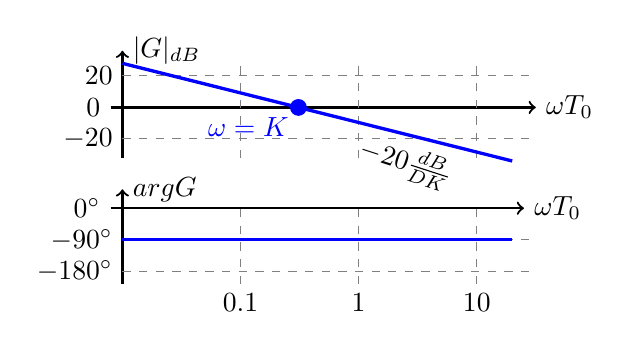
\begin{tikzpicture}[xscale=1.5, yscale=0.8]
	%% Amplitude
\begin{scope}
	%% Koordinatensystem
	\draw[thick, ->] (0,-1.2) -- (0,0.5) node[right] {$|G|_{dB}$};
	\draw[thick, ->] (-0.1,-0.4) node[left] {$0$} -- +(3.6,0) node[right] {$\omega T_0$};
	\draw[dashed,gray] (0,-0.9) node[left, black] {$-20$} -- +(3.5,0);
	\draw[dashed,gray] (0,0.1) node[left, black] {$20$} -- +(3.5,0);
	\draw[dashed,gray] (1,-1.2) -- +(0,1.5);
	\draw[dashed,gray] (2,-1.2) -- +(0,1.5);
	\draw[dashed,gray] (3,-1.2) -- +(0,1.5);
	%%%%%%%%%%%%%%%%

	%% Amplitudengang
	\draw[blue, very thick] (0,0.3) -- +(3.3,-1.55) node[near end, below, rotate=-18, black] {$-20\frac{dB}{DK}$};
	\draw(1.49,-0.4) node[draw,circle,inner sep=2pt,fill, blue] {};
	\node at (1.49, -0.4) [anchor = north east, blue] {$\omega = K$};
	
\end{scope}


%% Phase
\begin{scope}[shift={(0,-2.2)}]
	%% Koordinatensystem
	\draw[thick, ->] (-0.1,0.2) node[left] {$0^\circ$} -- +(3.5,0) node[right] {$\omega T_0$};
	\draw[thick, ->] (0,-1) -- (0,0.5) node[right] {$argG$};
	\draw[dashed,gray] (0,-0.3) node[left, black] {$-90^\circ$} -- +(3.5,0);
	\draw[dashed,gray] (0,-0.8) node[left, black] {$-180^\circ$} -- +(3.5,0);
	\draw[dashed, gray] (1,-1) node[below, black] {$0.1$} -- +(0,1.2);
	\draw[dashed,gray] (2,-1) node[below, black] {$1$} -- +(0,1.2);
	\draw[dashed,gray] (3,-1) node[below, black] {$10$} -- +(0,1.2);
	%%%%%%%%%%%%%%%%

	%% Amplitudengang
	\draw[blue, very thick] (0,-0.3) -- +(3.3,0);
\end{scope}

%\draw (current bounding box.south west) rectangle (current bounding box.north east);
\end{tikzpicture}